\documentclass[12pt]{article}
\pagestyle{plain}
\usepackage{xcolor}
\usepackage{lipsum}
\usepackage{setspace}
\renewcommand{\baselinestretch}{1.25} 
\usepackage{calc}
\usepackage{graphicx} 
\reversemarginpar
   \usepackage{graphicx}
\usepackage[paper=letterpaper, 
            marginparwidth=0.1in, 
            marginparsep=.1in, 
            margin=0.9in,
            left=0.9in,%
            right=0.9in,%
            includemp]{geometry}

\setlength{\parindent}{0in}

\usepackage[shortlabels]{enumitem}
% ============================================================
%:Markup macros for proof-reading
\usepackage{ifthen}
\usepackage[normalem]{ulem} % for \sout
\usepackage{xcolor}
\newcommand{\ra}{$\rightarrow$}
\newboolean{showedits}
\setboolean{showedits}{true} % toggle to show or hide edits
%\setboolean{showedits}{false} % toggle to show or hide edits
\ifthenelse{\boolean{showedits}}
{
	\newcommand{\meh}[1]{\textcolor{red}{\uwave{#1}}} % please rephrase
	\newcommand{\ins}[1]{\textcolor{blue}{\uline{#1}}} % please insert
	\newcommand{\del}[1]{\textcolor{red}{\sout{#1}}} % please delete
	\newcommand{\chg}[2]{\textcolor{red}{\sout{#1}}{\ra}\textcolor{blue}{\uline{#2}}} % please change
	\newcommand{\nbe}[3]{
		{\colorbox{#3}{\bfseries\sffamily\scriptsize\textcolor{white}{#1}}}
		{\textcolor{#3}{\sf\small$\blacktriangleright$\textit{#2}$\blacktriangleleft$}}}
}{
	\newcommand{\meh}[1]{#1} % please rephrase
	\newcommand{\ins}[1]{#1} % please insert
	\newcommand{\del}[1]{} % please delete
	\newcommand{\chg}[2]{#2}
	\newcommand{\nbe}[3]{}
}
%
\newcommand\rA[1]{\nbe{Reviewer A}{#1}{cyan}}
\newcommand\rB[1]{\nbe{Reviewer B}{#1}{olive}}
\newcommand\rC[1]{\nbe{Reviewer C}{#1}{magenta}}
\newcommand\ANS[1]{\nbe{Response}{#1}{teal}}
% ============================================================
%:Put edit comments in a really ugly standout display
%\usepackage{ifthen}
\usepackage{amssymb}
\newboolean{showcomments}
\setboolean{showcomments}{true}
%\setboolean{showcomments}{false}
\newcommand{\id}[1]{$-$Id: scgPaper.tex 32478 2010-04-29 09:11:32Z oscar $-$}
\newcommand{\yellowbox}[1]{\fcolorbox{gray}{yellow}{\bfseries\sffamily\scriptsize#1}}
\newcommand{\triangles}[1]{{\sf\small$\blacktriangleright$\textit{#1}$\blacktriangleleft$}}
\ifthenelse{\boolean{showcomments}}
%{\newcommand{\nb}[2]{{\yellowbox{#1}\triangles{#2}}}
{\newcommand{\nbc}[3]{
 {\colorbox{#3}{\bfseries\sffamily\scriptsize\textcolor{white}{#1}}}
 {\textcolor{#3}{\sf\small$\blacktriangleright$\textit{#2}$\blacktriangleleft$}}}
 \newcommand{\version}{\emph{\scriptsize\id}}}
{\newcommand{\nbc}[3]{}
 \newcommand{\version}{}}
\newcommand{\nb}[2]{\nbc{#1}{#2}{orange}}
\newcommand{\here}{\yellowbox{$\Rightarrow$ CONTINUE HERE $\Leftarrow$}}
\newcommand\rev[2]{\nb{TODO (rev #1)}{#2}} % reviewer comments
\newcommand\fix[1]{\nb{FIX}{#1}}
\newcommand\todo[1]{\nb{TO DO}{#1}}
\newcommand\on[1]{\nbc{ON}{#1}{red}} % add more author macros here
%\newcommand\XXX[1]{\nbc{XXX}{#1}{blue}}
%\newcommand\XXX[1]{\nbc{XXX}{#1}{brown}}
%\newcommand\XXX[1]{\nbc{XXX}{#1}{cyan}}
%\newcommand\XXX[1]{\nbc{XXX}{#1}{darkgray}}
%\newcommand\XXX[1]{\nbc{XXX}{#1}{gray}}
%\newcommand\XXX[1]{\nbc{XXX}{#1}{magenta}}
%\newcommand\XXX[1]{\nbc{XXX}{#1}{olive}}
%\newcommand\XXX[1]{\nbc{XXX}{#1}{orange}}
%\newcommand\XXX[1]{\nbc{XXX}{#1}{purple}}
%\newcommand\XXX[1]{\nbc{XXX}{#1}{red}}
%\newcommand\XXX[1]{\nbc{XXX}{#1}{teal}}
%\newcommand\XXX[1]{\nbc{XXX}{#1}{violet}}
% ============================================================


\makeatletter
\newlength{\bibhang}
\setlength{\bibhang}{1em}
\newlength{\bibsep}
 {\@listi \global\bibsep\itemsep \global\advance\bibsep by\parsep}
\newlist{bibsection}{itemize}{3}
\setlist[bibsection]{label=,leftmargin=\bibhang,%
        itemindent=-\bibhang,
        itemsep=\bibsep,parsep=\z@,partopsep=0pt,
        topsep=0pt}
\newlist{bibenum}{enumerate}{3}
\setlist[bibenum]{label=[\arabic*],resume,leftmargin={\bibhang+\widthof{[99]}},%
        itemindent=-\bibhang,
        itemsep=\bibsep,parsep=\z@,partopsep=0pt,
        topsep=0pt}
\let\oldendbibenum\endbibenum
\def\endbibenum{\oldendbibenum\vspace{-.6\baselineskip}}
\let\oldendbibsection\endbibsection
\def\endbibsection{\oldendbibsection\vspace{-.6\baselineskip}}
\makeatother


\usepackage{fancyhdr,lastpage}
\pagestyle{fancy}
%\pagestyle{empty}      % Uncomment this to get rid of page numbers
\fancyhf{}\renewcommand{\headrulewidth}{0pt}
\fancyfootoffset{\marginparsep+\marginparwidth}
\newlength{\footpageshift}
\setlength{\footpageshift}
          {0.2\textwidth+0.2\marginparsep+0.2\marginparwidth-2in}
%\lfoot{\hspace{\footpageshift}%
%       \parbox{2in}{\, \hfill %
%                    \arabic{page} of \protect\pageref*{LastPage} % +LP
%%                    \arabic{page}                               % -LP
%                    \hfill \,}}

% Finally, give us PDF bookmarks
\usepackage{color,hyperref}
\definecolor{darkblue}{rgb}{0.0,0.0,0.3}
\hypersetup{colorlinks,breaklinks,
            linkcolor=darkblue,urlcolor=darkblue,
            anchorcolor=darkblue,citecolor=darkblue}


\newcommand{\makeheading}[2][]%
        {\hspace*{-\marginparsep minus \marginparwidth}%
         \begin{minipage}[t]{\textwidth+\marginparwidth+\marginparsep}%
             {\large \bfseries #2 \hfill #1}\\[-0.15\baselineskip]%
                 \rule{\columnwidth}{1pt}%
         \end{minipage}}

\renewcommand{\section}[1]{\pagebreak[3]%
    \vspace{1.3\baselineskip}%
    \phantomsection\addcontentsline{toc}{section}{#1}%
    \noindent\llap{\scshape\smash{\parbox[t]{\marginparwidth}{\hyphenpenalty=10000\raggedright #1}}}%
    \vspace{-\baselineskip}\par}

\newcommand*\fixendlist[1]{%
    \expandafter\let\csname preFixEndListend#1\expandafter\endcsname\csname end#1\endcsname
    \expandafter\def\csname end#1\endcsname{\csname preFixEndListend#1\endcsname\vspace{-0.6\baselineskip}}}

\let\originalItem\item
\newcommand*\fixouterlist[1]{%
    \expandafter\let\csname preFixOuterList#1\expandafter\endcsname\csname #1\endcsname
    \expandafter\def\csname #1\endcsname{\csname preFixOuterList#1\endcsname\let\oldItem\item\def\item{\pagebreak[2]\oldItem}}
    \expandafter\let\csname preFixOuterListend#1\expandafter\endcsname\csname end#1\endcsname
    \expandafter\def\csname end#1\endcsname{\let\item\oldItem\csname preFixOuterListend#1\endcsname}}
\newcommand*\fixinnerlist[1]{%
    \expandafter\let\csname preFixInnerList#1\expandafter\endcsname\csname #1\endcsname
    \expandafter\def\csname #1\endcsname{\let\oldItem\item\let\item\originalItem\csname preFixInnerList#1\endcsname}
    \expandafter\let\csname preFixInnerListend#1\expandafter\endcsname\csname end#1\endcsname
    \expandafter\def\csname end#1\endcsname{\csname preFixInnerListend#1\endcsname\let\item\oldItem}}
 
\newlist{outerlist}{itemize}{3}
    \setlist[outerlist]{label=\enskip\textbullet,leftmargin=*}
    \fixendlist{outerlist}
    \fixouterlist{outerlist}

\newlist{lonelist}{itemize}{3}
    \setlist[lonelist]{label=\enskip\textbullet,leftmargin=*,partopsep=0pt,topsep=0pt}
    \fixendlist{lonelist}
    \fixouterlist{lonelist}

\newlist{innerlist}{itemize}{3}
    \setlist[innerlist]{label=\enskip\textbullet,leftmargin=*,parsep=0pt,itemsep=0pt,topsep=0pt,partopsep=0pt}
    \fixinnerlist{innerlist}

\newlist{loneinnerlist}{itemize}{3}
    \setlist[loneinnerlist]{label=\enskip\textbullet,leftmargin=*,parsep=0pt,itemsep=0pt,topsep=0pt,partopsep=0pt}
    \fixendlist{loneinnerlist}
    \fixinnerlist{loneinnerlist}

\newcommand{\blankline}{\quad\pagebreak[3]}
\newcommand{\halfblankline}{\quad\vspace{-0.5\baselineskip}\pagebreak[3]}

\newcommand\doilink[1]{\href{http://dx.doi.org/#1}{#1}}
\newcommand\doi[1]{doi:\doilink{#1}}

\providecommand*\url[1]{\href{#1}{#1}}
\renewcommand*\url[1]{\href{#1}{\texttt{#1}}}
\providecommand*\email[1]{\href{mailto:#1}{#1}}
\providecommand\BibTeX{{B\kern-.05em{\sc i\kern-.025em b}\kern-.08em
    \TeX}}
\providecommand\Matlab{\textsc{Matlab}}
\hyphenation{bio-mim-ic-ry bio-in-spi-ra-tion re-us-a-ble pro-vid-er}

\pagenumbering{roman}

\begin{document}
\pagenumbering{roman}
%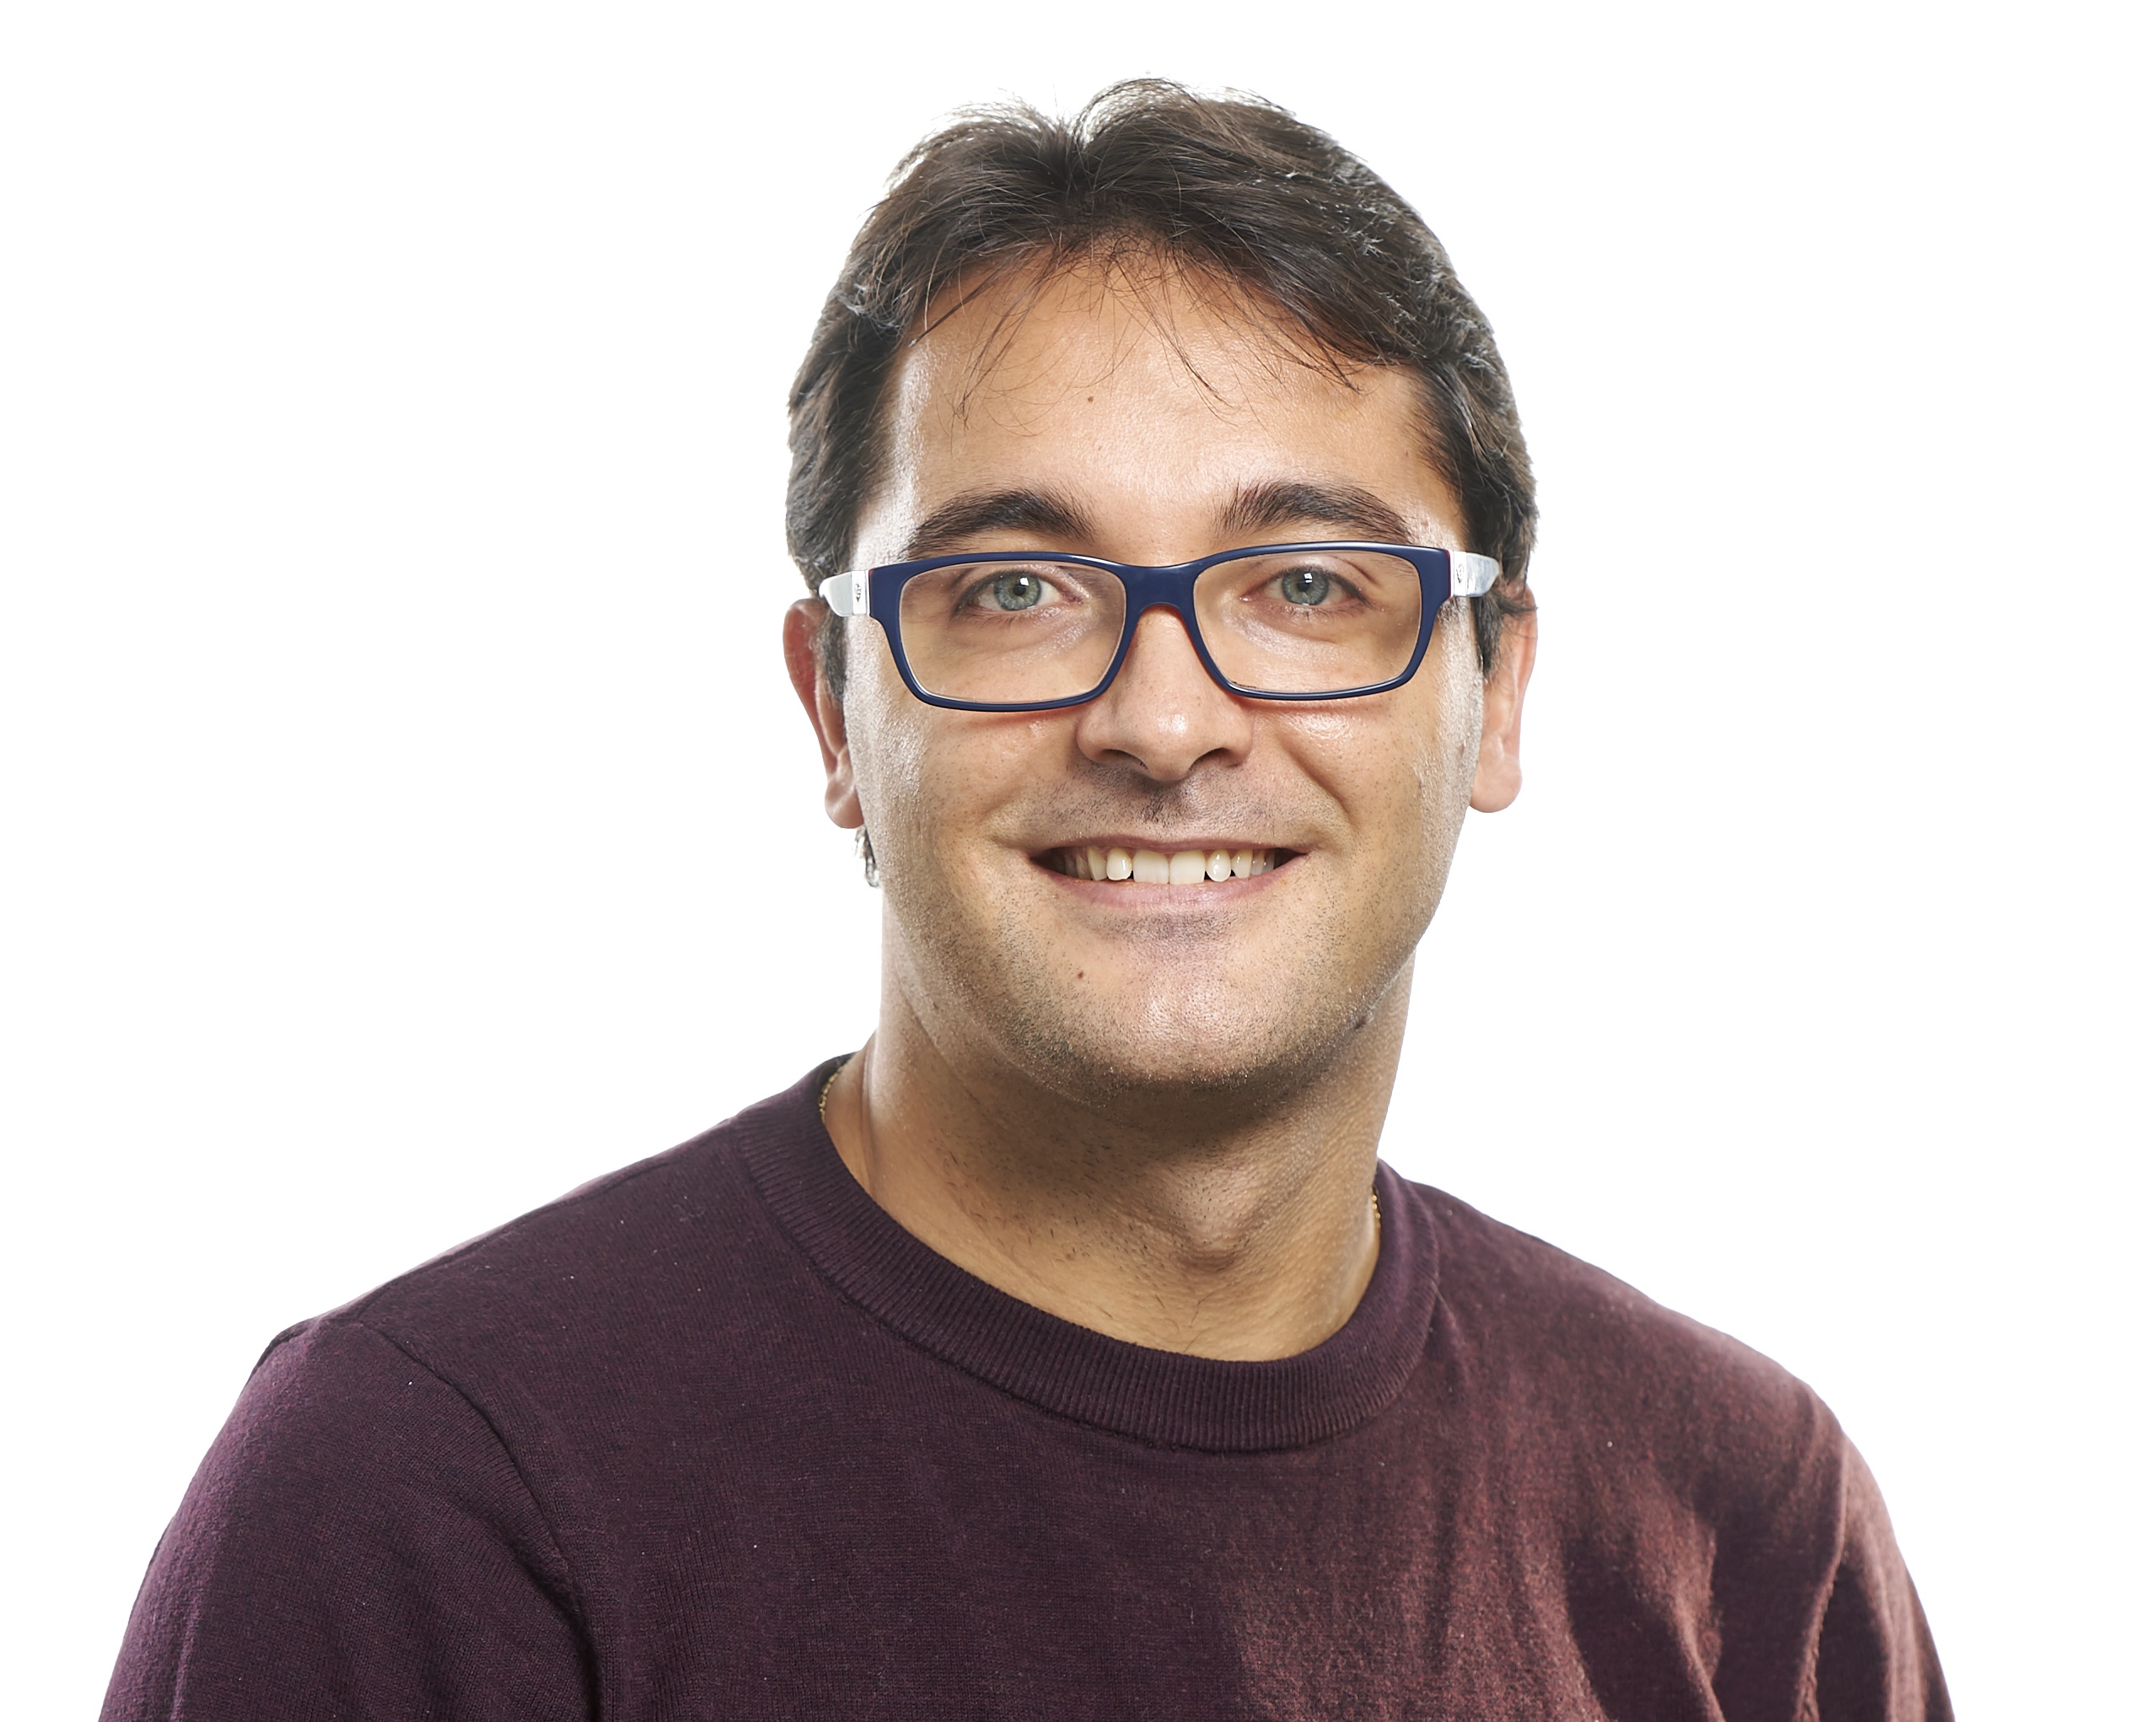
\includegraphics[width=3.3cm, height=3.5cm]{images/s_panichella.jpg}\\
\vspace{-2mm}
\textsc{Sebastiano Panichella - Curriculum vitae}\\
\vspace{-2mm}

%\newlength{\rcollength}\setlength{\rcollength}{1in}%
%\newlength{\spacewidth}\setlength{\spacewidth}{20pt}
%\newcommand\spacechar{$|$}

\noindent\begin{minipage}{0.3\textwidth}% adapt widths of minipages to your needs
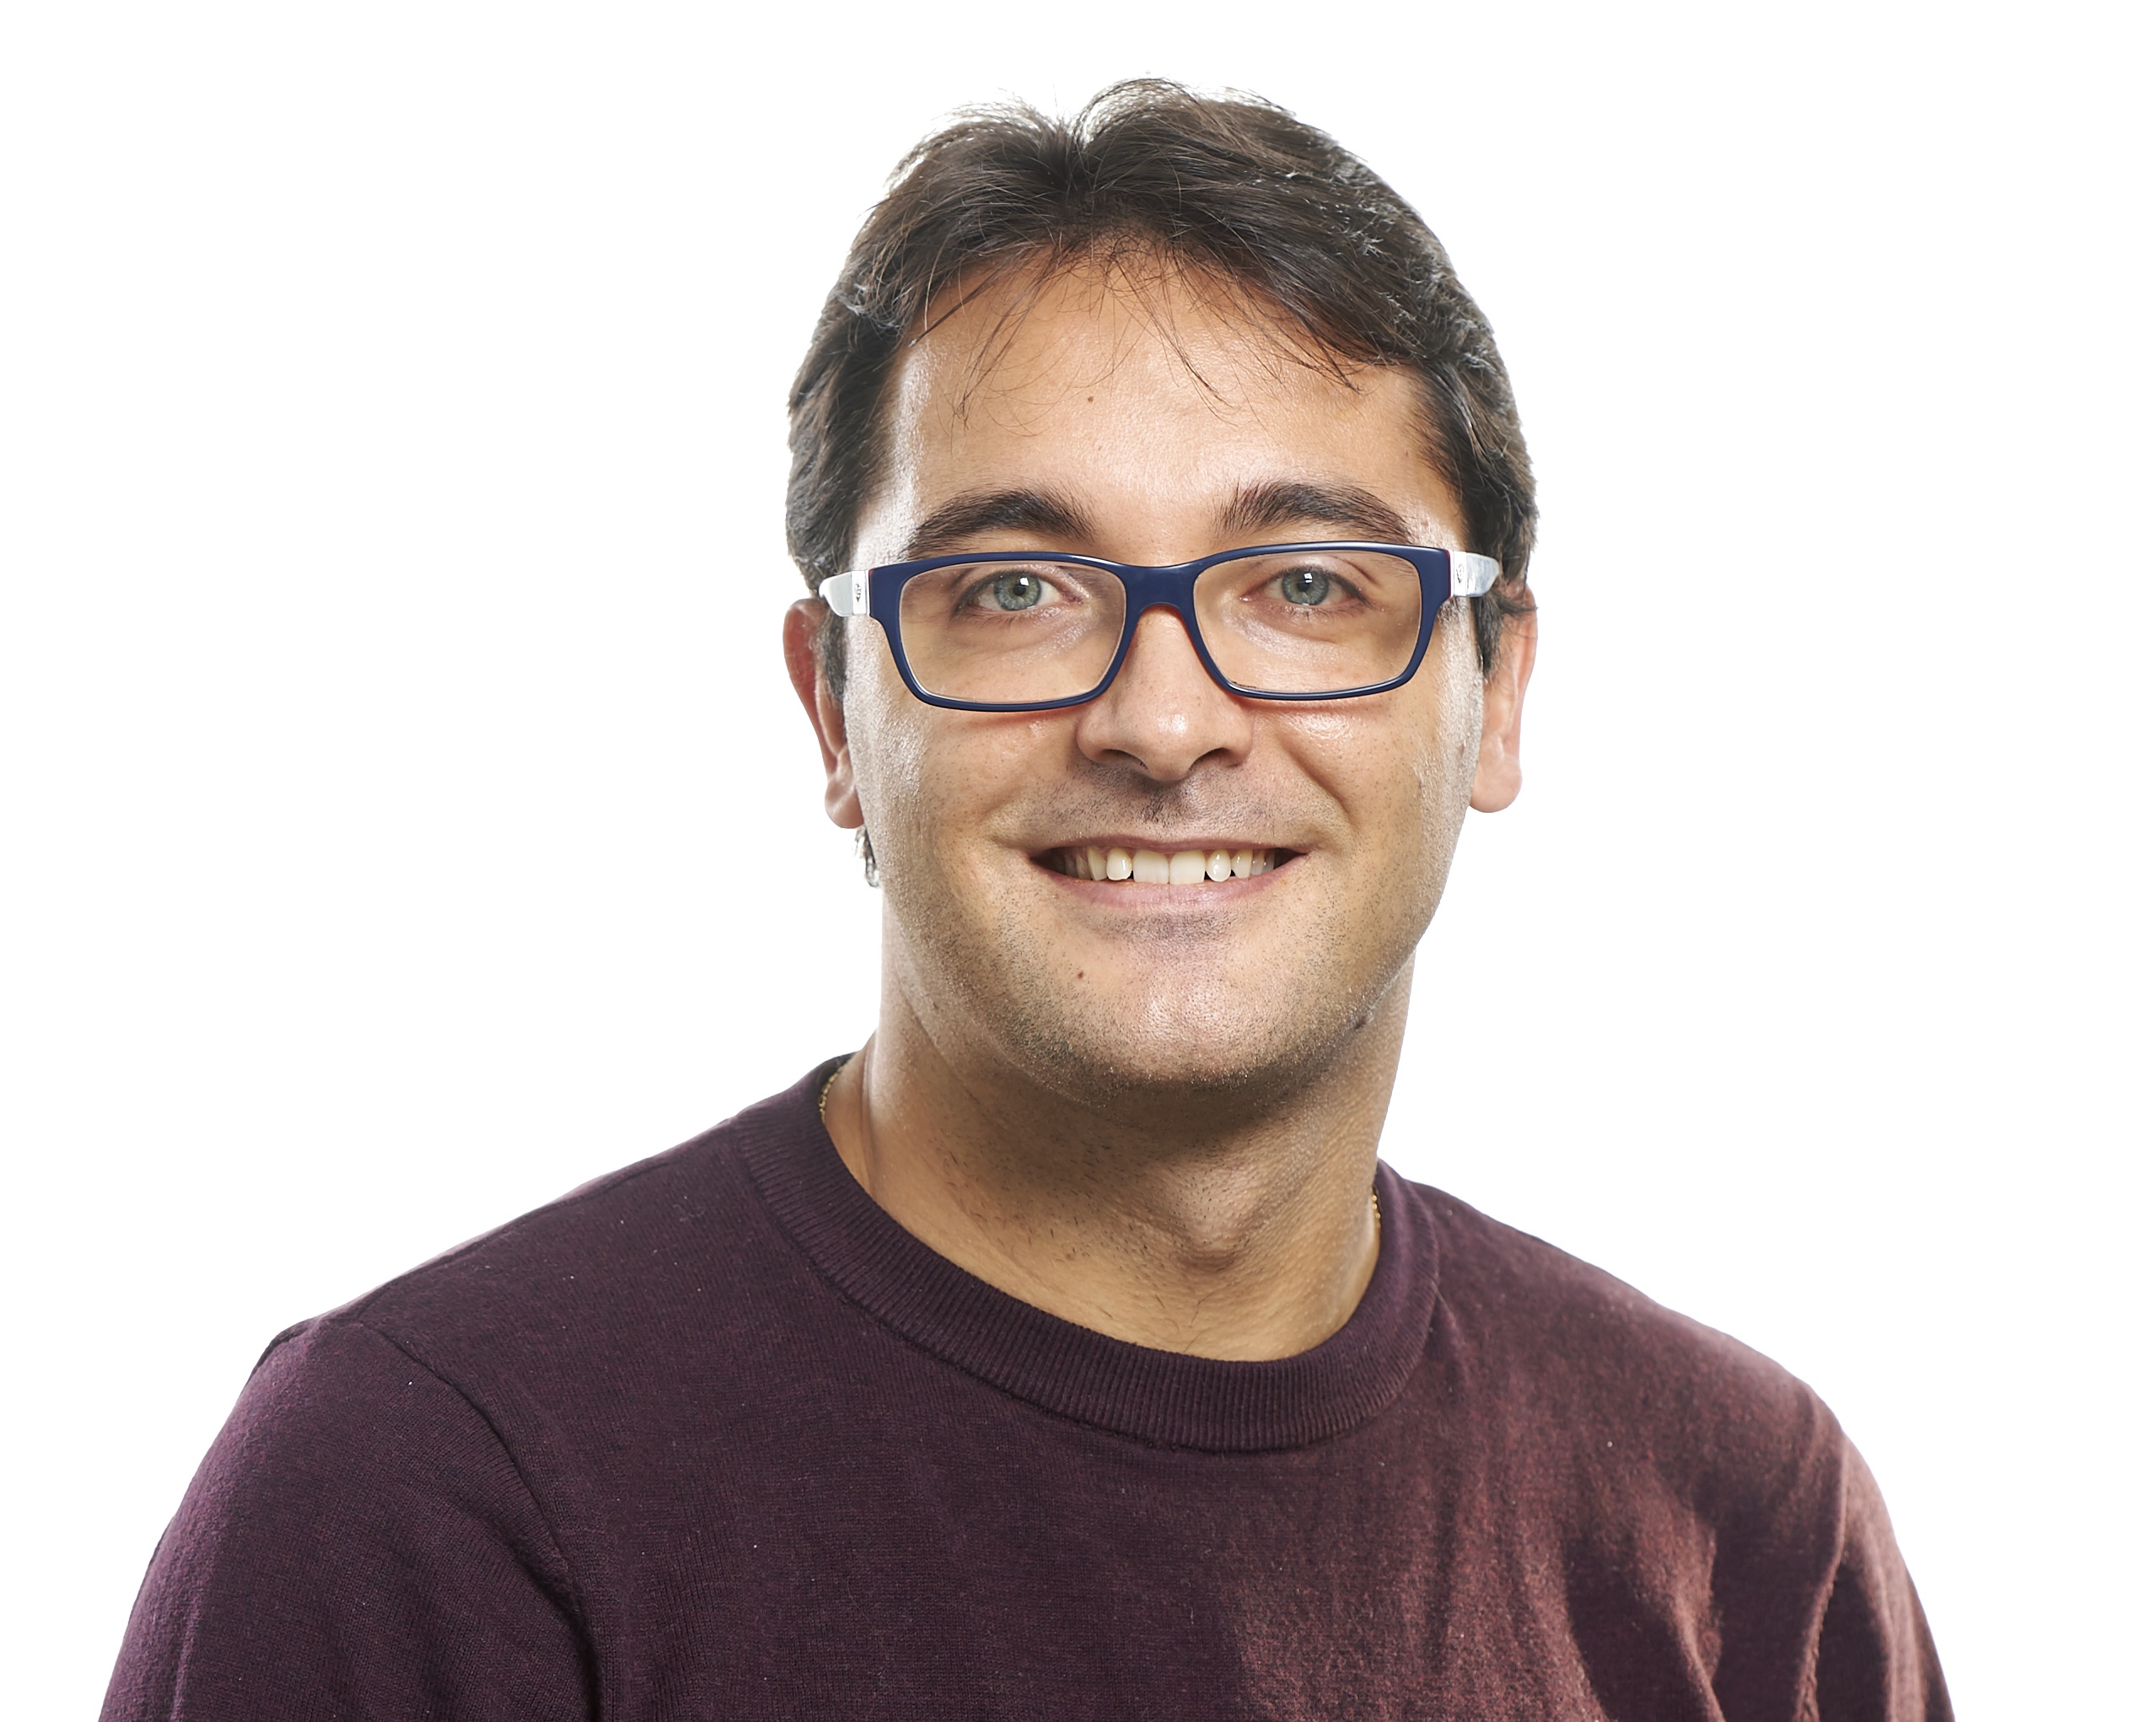
\includegraphics[width=3.9cm, height=3.5cm]{images/s_panichella.jpg}
\end{minipage}%
\hfill%
\begin{minipage}{0.9\textwidth}\raggedright
\textsc{Contact Information}\\
{\small
%\textit{Address:} Department of Computer Engineering\\ \href{http://www.ing.unisannio.it/}{University of Sannio}\\
%RCOST- Palazzo ex Poste, Via Traiano\\
%82100 Benevento (Italy).\\\\
%\textit{Mobile:} +39 3881969673\\
%\textit{Tel.: +39 0824 305539} \\
%\textit{E-mail:} \email{spanichella@gmail.com}\\
%\textit{Home Page:} \href{http://www.ing.unisannio.it/spanichella}{www.ing.unisannio.it/spanichella}
\textit{Address:} School of Engineering,  \href{https://www.zhaw.ch/en/about-us/person/panc/}{Zurich University of Applied Science}\\
Obere Kirchgasse 2 / Steinberggasse 12/14
8400 Winterthur, Switzerland.\\
%\textit{Office: BIN 2.D.03}
%\\ %\textit{Mobile:} +41 788864624\\
%\textit{Tel.: +39 0824 305539} \\
%\textit{Tel +41 44 63 545 78 } \\
\textit{E-mail:} \email{panc@zhaw.ch} (or alternatively \email{spanichella@gmail.com})\\
\textit{Home Page:} \href{https://spanichella.github.io/index.html}{https://spanichella.github.io/index.html}\\
\textit{Google Scholar Ref:}  \url{https://scholar.google.it/citations?user=HiNuBFgAAAAJ\&hl=en\&oi=ao}\\
\textit{Detailed CV:} \href{https://spanichella.github.io/img/CV.pdf}{https://spanichella.github.io/img/CV.pdf}}\\
\end{minipage}


\vspace{2.5mm}
\textsc{EDUCATION}
\vspace{1.5mm}

Sebastiano Panichella was born (19/12/1986) 
in Isernia (Italy), he received (cum laude) the Laurea in Computer Science from the University of Salerno (Italy) in December 2010 defending a thesis on IR-based Traceability Recovery. 
He received the PhD in Computer Science from the University of Sannio (Department of Engineering) defending, in  \textbf{18 July 2014},  the thesis entitled  \href{http://dx.doi.org/10.1109/ICSM.2015.7332519}{\textit{``Supporting Newcomers in Open Source Software Development Projects"}}.  During the PhD his work was supervised by \textbf{\textit{Prof. Massimiliano Di Penta and Prof. Gerardo Canfora}}.

\vspace{2.5mm}
\textsc{Employment history \& Research Goals and Interests}
\vspace{1.5mm}
%During the PhD his work was supervised by 
%Prof. Gerardo Canfora and 
%Prof. Massimiliano Di Penta and Prof. Gerardo Canfora.

%\textbf{Major scientific achievements}
%\vspace{1mm}

Currently he is a (Permanent) Senior Computer Science Researcher at Zurich University of Applied Science (from \textit{\textbf{20-08-2018}}) and Part-time (External) Lecturer at the University of Zurich (from \textit{\textbf{20-08-2018}}). Previously he was postdoc at University of Zurich (01-11-2014 - 19-08-2018) working in the lab of Prof. Gall. \\\\
His main \textbf{research goal} is to conduct industrial research, involving both industrial and academic collaborations, to sustain
the Internet of Things (IoT) vision, where future smart cities will be characterized by millions of smart systems (e.g., cyber-physical
systems) connected over the internet, controlled by complex embedded software implemented for the cloud.\\
His  \textbf{research interests} are in the domain of Software Engineering (SE), cloud computing (CC), and Data Science (DS): DevOps (e.g., Continuous Delivery, Continuous integration), Machine learning applied to SE, Software maintenance and evolution (with particular focus on Cloud, mobile, AI-based, and Cyber-physical applications). Moreover, he is promoting DS research on \href{https://doi.org/10.1109/VST.2018.8327148}{\textit{Summarization Techniques for Code, Changes, and Testing}}. He is a \textbf{member of IEEE}. 
\vspace{1mm}

He authored or co-authored more than \textbf{seventy} (considering also demonstration, dataset 
  and poster) papers appeared in International Conferences and Journals (26 of them published during the postdoctoral experience at the SEAL lab). His research projects involved relevant industrial companies (e.g., ING NEDERLAND, Sony Mobile Communication, SIEMENS, GVM, etc.) and their extensions will involve further industrial organizations and open source projects. He serves and has served as \href{https://spanichella.github.io/\#services}{program committee member} of various international conference (e.g., ICSE, SBST, ASE, ICPC, ICSME, SANER, MSR, SEAA) and as \href{https://spanichella.github.io/\#services}{reviewer for various international journals} (e.g., TSE, TOSEM, EMSE, JSS, IST, JSEP) in the fields of software engineering and evolutionary computation. He is currently Editorial Board Member of the \textit{Journal of Software: evolution and process} (JSEP) and in was recently \href{https://spanichella.github.io/\#services}{Lead (or Co-lead) Guest editor} of special issues at EMSE and IST journals.\\

\vspace{1.5mm}
\textsc{Institutional responsibilities}
\vspace{1.5mm}

(Permanent) Senior Computer Science Researcher in Software Engineering (SE), cloud computing (CC), and Data Science (DS) at ZHAW (from 20-08-2018) and Part-time (External) Lecturer at the University of Zurich (from \textit{20-08-2018}).

\vspace{2.5mm}
\textbf{Internships}
\begin{innerlist}
   \item \emph{
              \href{http://www.polymtl.ca/‎}
                   {May-July 2013 was visiting researcher at the Ecole Polytechnique de Montr\`{e}al, Canada. Supervisor: Prof. Giuliano Antoniol}}
\end{innerlist}
\vspace{5.5mm}

\textsc{Approved research projects}
\vspace{1.5mm}


%\on{Why are you using href for the entire text?}\\
\textbf{EU projects}
\begin{innerlist}
\item Sebastiano Panichella is the technical coordinator for the EU H2020-ICT-2018-20 call, entitled COSMOS, contract no. 957254. \textbf{Description}: Much of the increasing complexity of ICT systems is being driven by the more distributed and heterogeneous nature of these systems, with Cyber-Physical Systems accounting for an increasing portion of Software Ecosystems. This basic premise underpins the COSMOS proposal which focuses on blending best practices DevOps solutions with the development processes used in the CPS context: this will enable the CPS world to deliver software more rapidly and result in more secure and trustworthy systems. 
 %COSMOS brings together a balanced consortium of big industry, SMEs and academics which will develop enhanced DevOps pipelines which target development of CPS software.
The COSMOS CPS pipelines will be validated against 5 use cases provided by industrial partners representing healthcare, avionics, automotive, utility and railway sectors.  
\textbf{Total H2020 project 5MIL EUR, Sebastiano Panichella got direct funding for 770,000 EUR} 
   \item Sebastiano Panichella was 
   %\ins{was}
    partially funded with Gabriele Bavota, Gerardo Canfora, Massimiliano Di Penta, in the \href{��http://www.markosproject.eu/��}
                   {EU FP7-ICT-2011-8 project Markos}, contract no. 317743. Specifically, the MARKOS project aimed to realize the prototype of a service and an interactive application providing an integrated view on the Open Source projects available the on web, focusing on functional, structural and licenses aspects of software code. 
\end{innerlist}
\newpage
\textbf{Innosuisse projects}
\begin{innerlist}
   \item Sebastiano Panichella is the main research responsible of Innosuisse project ARIES: Exploiting User Journeys and Testing Automation for Supporting Efficient Energy Service Platforms (project Nr. 45548.1 IP-ICT).
ARIES brings together a consortium of two partners: the start-up LEDCity (\href{https://ledcity.io/}{https://ledcity.io/}) and the ZHAW. 
ARIES project delivers a data oriented and software platform that implements requirements and testing engineering mechanisms to enhance customer experience. ARIES project is realized in the context of LEDCity, a Swiss start-up specialized in AI-based optimization of lighting systems.\\
\textbf{Total project funding:} Sebastiano Panichella got direct funding for around \textbf{500,000 CHF}\\
%\textbf{Ack:} We personally thank the team of BOND for the very productive and constant research meetings. 
\end{innerlist}

\textbf{SNF projects}
\begin{innerlist}
   \item Sebastiano Panichella obtained funding  (as co-applicant) for
   %\chg{funded}{obtained funding for} 
   the SURF-MobileAppsData SNF (No. 200021$-$166275) project. The goal of the SURF-MobileAppsData project is mining mobile apps data available in app stores to support software engineers in better supporting maintenance and evolution activities for these apps (\textbf{Total SNSF (CHF) 349,926}). \\See page: \href{http://www.ifi.uzh.ch/en/seal/people/panichella/SNF-Projects.html}{http://www.ifi.uzh.ch/en/seal/people/panichella/SNF-Projects.html}
\end{innerlist}

\vspace{6.5mm}


\textsc{Supervision (or Co-Supervision) of junior researchers at graduate and postgraduate level:}\\\\
He is \textbf{supervising, supervised (or co-supervised)} 11 undergrad students, 12 MSc students, 5 research assistants, and 9 PhD students (6 of them during the postdoctoral experience at the University of Zurich), which published in relevant conference and journal venues in Software Engineering. A more complete and updated information on advised researchers at different levels can be found: \href{https://spanichella.github.io/\#teaching}{https://spanichella.github.io/\#teaching}\\
\vspace{1.5mm}

\vspace{2.5mm}

\textsc{Awards}
\vspace{3.5mm}

\textbf{Award as Reviewer}: Distinguished Reviewer Award SATToSE 2017 and SANER 2018.


%\footnote{In papers marked with (*)  the authors are listed in alphabetic order}: %When such a rule is not followed, authors are listed by contribution.
\textbf{Best paper award:} ICPC 2011, MaLTeSQuE 2018.\\ 
\textbf{Best tool award}: ICPC 2014, SANER 2018. 

\vspace{1.5mm}

\textbf{Nominations for Best Paper}: ICSME 2020, ICSSP 2020, (2) SANER 2018, SANER 2017, ICSME 2014, ICPC 2014, ICSM 2013, ICST 2013.

\vspace{6.5mm}

\textsc{Major scientific achievements}

\vspace{-2.5mm}
\begin{itemize}
  \item According to the [Results reported by the JSS journal] Sebastiano Panichella was selected in 2021, according to the results reported by the JSS journal \footnote{https://www.sciencedirect.com/science/article/abs/pii/S0164121221001266}, as one of the \textbf{top-20 Most impactful SE researchers Worldwide in Software Engineering (SE)}. 
  \item According to the [Results reported by the JSS journal] Sebastiano Panichella was selected in 2019, according to the results reported by the JSS journal \footnote{https://www.sciencedirect.com/science/article/pii/S0164121218302334}, as one of the \textbf{top-20 Most Active Early Stage Researchers Worldwide in Software Engineering (SE)}. 
\vspace{-1.5mm}
  \item The paper [Sebastiano Panichella, Andrea Di Sorbo, Emitza Guzman, Corrado Aaron Visaggio, Gerardo Canfora, Harald C. Gall: How can I improve my app? Classifying user reviews for software maintenance and evolution. ICSME 2015: 281-290], which originated the idea behind this SNF project, is one of the \textbf{most cited papers of ICMSE 2015} (as reported in Google scholar), with over 370 citations in around 5-6 years.
  \item The research proposal submitted to the H2020 grant called COSMOS: ``DevOps for Complex Cyber-physical Systems" was recently selected for funding.
  \item The research proposal submitted to the Innosuisse called ``ARIES: Exploiting User Journeys and Testing Automation for Supporting Efficient Energy Service Platforms" was recently selected for funding.
\vspace{-1.5mm}
  \item The paper ICPC wrote during the bachelor studies of Dr. Panichella-[Giovanni Capobianco, Andrea De Lucia, Rocco Oliveto, Annibale Panichella, Sebastiano Panichella: On the role of the nouns in IR-based traceability recovery. ICPC 2009: 148-157] is \textbf{among the most influential papers of ICPC in the last decade [period 2009-2019]}.
  \vspace{-1.5mm}
\end{itemize}

\textsc{Memberships in panels, boards, and individual scientific reviewing activities}

\vspace{3.5mm}

\textbf{Member of associations:}
\begin{innerlist}
\item Member of the EU Sparc Robotics group - https://sparc-robotics-portal.eu
\end{innerlist}

\textbf{Keynote Speaker of International Conferences and co-located events:}
\begin{innerlist}
\item Speaker at the \href{https://safecomp2021.hosted.york.ac.uk/wp-content/uploads/2021/08/DepDevOps_2021_programme.pdf}{Workshop on Dependable DevOps} co-located with the SafeComp conference, 2021.
\item Speaker at the Workshop on Validation, Analysis and Evolution of Software Tests - VST 2018  (http://vst2018.scch.at/\#program) 
\end{innerlist}

\textbf{Editor of special Issues at International Journals:}
\begin{innerlist}
\item Editor of Software Track special Issue at Journal of Science of Computer Programming on NLP-based software engineering. 2022.
\item Editor of a the special Issue at EMSE Journal entitled 'Software Engineering for Mobile Applications', July 2018.
\item Editor of a the special Issue at IST Journal entitled 'User Feedback and Software Quality in the Mobile Domain',  June 2018.
	
\end{innerlist}

\textbf{Organising research workshops:}
\begin{innerlist}
\item Chair of the \textit{Workshop on Natural Language-Based Software Engineering Workshop} (NLBSE) - Collocated with ICSE 2022
\item Chair of  the \textit{Workshop on Search-Based Software Testing} (SBST) - Collocated with ICSE 2022
\item Chair of the \textit{Workshop on DevOps Testing for Cyber-Physical Systems - Collocated with ICST 2021 \\(https://devops4cps-testing.github.io/)} 
\item \href{}
{Chair of the Tool Competition at the 
International Workshop on Search-Based Software Testing (SBST 2020 and 2021)} 
       \item \emph{\href{http://cnax.servicelaboratory.ch/}
                   {\textit{Chair of the first International Workshop on Cloud-Native Applications Design and Experience - CNAX 2018
Co-located with UCC 2018 and BDCAT 2018 conferences -}}, Zurich, Switzerland.}
\end{innerlist}

%\on{Get rid of all the emphasis (no italics needed).}\\
\textbf{Organising committee member of International Conferences and Workshops:}
\begin{innerlist}
 \item \href{https://spanichella.github.io/#services}{\textit{Program Committee member}} of ICSE, FSE, ASE, ICSME, ICST, ICSOFT, SSBSE, ICPC, SSBSE, SBST, SANER, MSR, WAISE, MaLTeSQuE, SEAA, SATToSE, VST, RoSE, QUATIC.
 \end{innerlist}

%\textbf{Session Chair of International Conferences:}
%\begin{innerlist}

 %      \item \emph{\href{http://saner.aau.at/}
  %                 {\textit{of the 24th IEEE International Conference on Software Analysis, Evolution, and Reengineering (SANER 2017)}}, Austria.}

%\end{innerlist}

%\textbf{Web Chair}
%\begin{innerlist}
  % \item \emph{
             % \href{http://icpc2014.usask.ca/‎}
                   %{21st International Conference on Program Comprehension %(ICPC 2013)}}, San Francisco, California, USA.\\
%\end{innerlist}

\textbf{Editorial Board Member of International Journals:}
\begin{innerlist}
   \item \emph{
              \href{http://onlinelibrary.wiley.com/journal/10.1002/(ISSN)2047-7481��}
                   {Journal of Software: evolution and process}}.
\end{innerlist}


\textbf{Reviewer for the following International Journals:}
\begin{innerlist}
\item \emph{Empirical Software Engineering - Transactions on Software Engineering - Transactions on Software Engineering and Methodology - Journal of Systems and Software - Information and Software Technology - Journal of Software: Evolution and Process - Science of Computer Programming - Journal of Computer Science and Technology - Transactions on Mobile Computing - Communications of the ACM - Software Testing, Verification and Reliability - Journal of Object Technology}\\
\end{innerlist} 



\textbf{External Reviewer of Grant Applications}
\begin{innerlist}
   \item \emph{
              \href{http://www.frqnt.gouv.qc.ca/accueil}
                   {External Reviewer of projects submitted in the Quebec-Flanders bilateral research cooperation program}}
\item \emph{
              \href{}
                   {External Reviewer of projects submitted in the Mitacs Accelerate research program}}
                   
\end{innerlist}


\textbf{Research Meetings}
\begin{innerlist}
   \item \emph{
              \href{http://www.nii.ac.jp/��}
                   {Sebastiano Panichella was invited by the \href{http://www.nii.ac.jp/}{National Institute of Informatics} (NII), Japan, to participate in \href{http://shonan.nii.ac.jp/shonan/}{NII Shonan Meeting entitled ``Mobile App Store Analytics"} (Japan).
}}

\item  \emph{Sebastiano Panichella was invited by the \href{http://www.adesso.de/de/}{Adesso company}, Switzerland, to participate in \textit{``Adesso Quartalsmeeting" 2016} (Zurich).}

\end{innerlist}
\vspace{8.5mm}


\textbf{RESEARCH PARTNERS \& COLLABORATIONS established in the last years}:\\
(\textcolor{blue}{collaborations summarized at \href{https://spanichella.github.io/\#collaborations}{https://spanichella.github.io/\#collaborations})}

\textbf{Collaboration with researchers in the supervision or co-supervision of PhD students and research assistants}:
 Currently, he is advising at the Zurich University of Applied Science (ZHAW), the PhD  work of Sajad Khatiri (with Paolo Tonella from University of Lugano) and other 3 research assistants, on research concerning DevOps for complex systems (funded in EU and national projects).
 With Prof. Oscar Nierstrasz he is also co-advising the research work of Pooja Rani, PhD student at University of Bern, Switzerland (from 2018), on topics concerning code comments analysis and assessment. In the past years, Dr. Panichella advised the work of a research assistant (Diego Martin) at the ZHAW, co-supervised with Prof. Gall the research work of 5 PhD students at the University of Zurich, 1 PhD student at the University of Sannio (Italy) with Prof. Gerardo Canfora, 1 at University of Chinese Academy of Sciences, Beijing, China (Laboratory for Internet Software Technologies).
 More information on his advising or co-advising experience can be found at \href{https://spanichella.github.io/\#teaching}{https://spanichella.github.io/\#teaching}

\textbf{Established Research partners interested to collaborate to projects and proposals with Dr. Panichella}: Timo Kehrer (University of Bern); Davide Scaramuzza (University of Zurich); Stefano Mintchev (ETH); Paolo Tonella (University of Lugano)
 University of Luxembourg, Dr. Bianculli and Dr. Pastore (Testing, Requirement engineering, and formal verification); Simula, Department of Engineering, Dr. Shaukat (Cyber-Physical Systems of Systems);  Delft University of Technology,
Dr. Zaidman (automated testing); Tampere University of Technology, Prof. Davide Taibi (DevOps, cloud computing); Prof.
Robles (Mining Software Repositories techniques). With most of the aforementioned (excluding Prof. Robles, that recently published
with us a paper at Onward 2018) partners we collaborate on strategic EU and national projects. 

\textbf{Collaborations with the industrial partners (via the involvement in research papers, projects and proposals)}:\\
- Siemens AG and Siemens Healthcare GmbH	Germany	2019-05-Today\\
- BOND	Switzerland	2019-10-Today\\
%- Helio	Switzerland	2019-10-Today\\
- Intelligentia S.r.l.	Italy	2020-01-Today\\
- AICAS GmbH	Germany	2020-01-Today\\
- Q-media s.r.o.	Czech Republic	2020-01-Today\\
- Unparallel Innovation LDA	Portugal	2019-01-Today\\
- The Open Group (Scott Hansen) Belgium 2019-01-Today\\
- GMV https://www.gmv.com Spain 2019-01-Today\\
- https://www.intelligentia.eu (Italy); 2019-01-Today\\
- DENSO https://www.denso.com/de/en/innovation/ 2019-01-Today\\
- Haidar Osman (Senior Data Scientist - Swisscom, Switzerland); 2018-Today
- Red Hat Switzerland 2018-Today\\
- https://vshn.ch/en/ Switzerland 2018-Today\\
- https://ikubinfo.al/ Austria 2018-Today\\
- Daniele Romano (ING Netherland); 2017-Today\\
- Junji Shimagaki (Sony Mobile Communications); 2016-2018\\
- etc.

\textbf{Established collaborations with Robotics labs \& Exploitation Plans:}\\
 Dr. Panichella is currently collaborating with Prof. Scaramuzza on research concerning robotics and software engineering, primary on the co-supervision of thesis in the intersection of software engineering and robotics systems development. He is also fostering collaborations with robotics experts at ZHAW, focused on drones development.
 Dr. Panichella plans to exploit tools and technologies developed in his research projects, involving industrial organizations in Switzerland (e.g., Red Hat), including companies
in which CPS and AI technologies are critical for their business. 
Dr. Panichella plan to disseminate his projects results within software engineering, robotics courses at the Bachelor/Master level, thus fostering
technological transfer to future employees of enterprises in the territory. Finally, Dr. Panichella is committed to establish the open source tools developed within his projects, to promote industrial and open source ecosystems and collaborations.\\

\textbf{TEACHING (UZH and ZHAW) activities \& Achievements:}\\
\textbf{University of Zurich:} \\
-   Lecturer and co-lecturer for the Software Maintenance and Evolution course in 2014, 2015, 2016, 2017, 2018, 2019, 2020, 2021\\   \textit{Learning Goals}: During the course Sebastiano teach to
the students the foundations of software evolution and maintenance, by integrating recent research in both cloud computing and
software engineering fields, thus transferring to students also this recent research outputs (in form of papers, datasets, tools and
prototypes). This includes successful aged (i.e. legacy software) or cloud-based software systems, object-oriented reengineering,
refactoring, change patterns, empirical analysis of software, classification/prediction models, software quality analysis.\\
\textbf{Zurich University of Applied Science (ZHAW):}\\
- Cloud Computing course - CCP2 2020\\
- INF-Prog1 2020. Learning Goals: The main features of the Python program language.\\
- Co-lecturer for the CAS Information Engineering in 2018, 2019, 2020.
Learning Goals: The main features of the Python program language.\\
- Lab Instructor for the Programming course in Java in 2018, 2019, 2020.
Learning Goals: The main features of the Java program language.\\


\href{http://www.unisa.it}{\textbf{University of Sannio}}:\\

- \textit{Lab Instructor} (December 2013) for the Programming Techniques course of Professor Gerardo Canfora\\   \textit{Learning Goals}:   The Languages ​​and Grammars, JavaCC parser.\\
- \textit{Teaching Assistant } for the Software Engineering course of Prof. Massimiliano Di Penta:\\   \textit{Learning Goals}:   
Recovering Traceability Links via Information Retrieval Methods\\


\textbf{DATASET \& TOOLS:}\\
A comprehensive and updated list of shared datasets/tools to the research community by Sebastiano is available at\\ https://spanichella.github.io/tools.html\\

\vspace{3.5mm}

\textsc{Spoken Languages}\\

Sebastiano Panichella currently speaks three languages: Italian (mather tongue), English (\textit{C1}) and German (\textit{A2.2}). He is actively studying German. Specifically, he started to study the German language in the last years. Thus, followed two courses at the UZH in the past. He recently followed, during the fall semester 2020, a course at ZHAW for reaching the B1 German level and successfully passed the final evaluation exam. He plans to continue his studies to reach the B2 level during the spring semester of 2022, to be able to reach a C1 level during the year 2023.


\halfblankline
\blankline



\end{document}
